\documentclass{article}
\usepackage{tikz}
\usetikzlibrary{arrows.meta}

\begin{document}

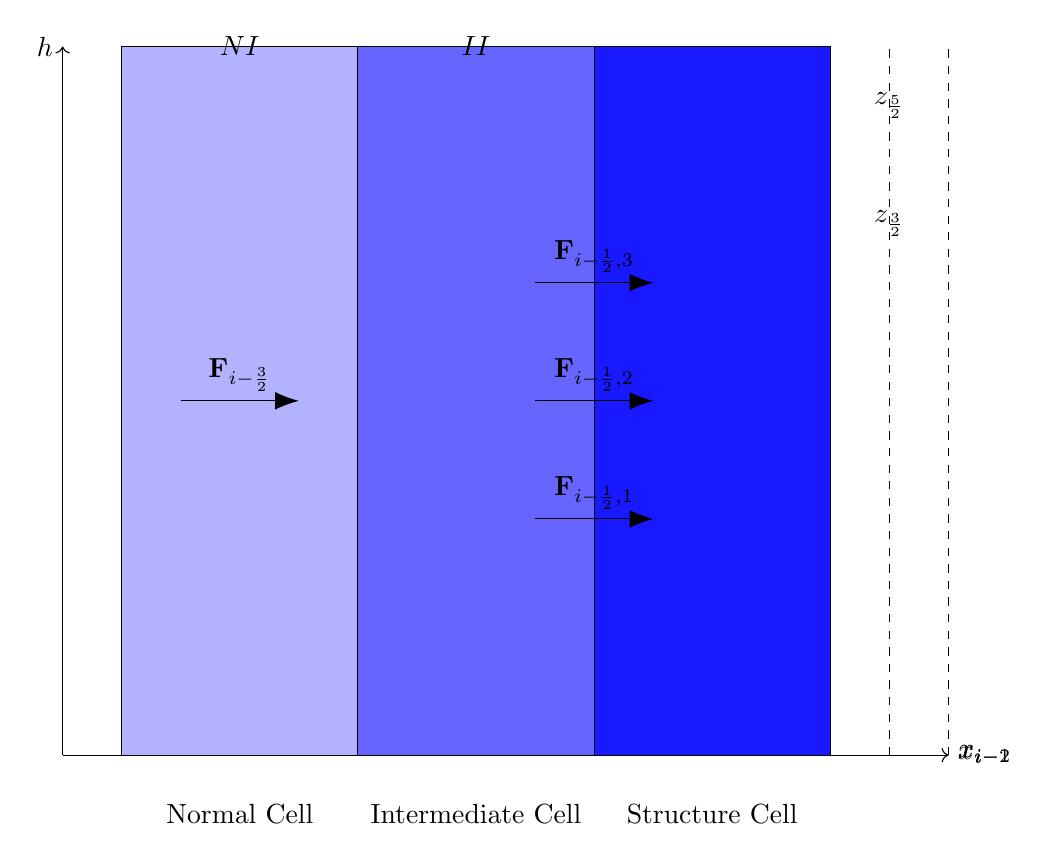
\begin{tikzpicture}[scale=1.5]
    % Draw the vertical lines
    \draw[dashed] (0,0) -- (0,6);
    \draw[dashed] (2,0) -- (2,6);
    \draw[dashed] (4,0) -- (4,6);
    
    % Draw the horizontal lines
    \draw[fill=blue!30] (0,0) rectangle (2,6);
    \draw[fill=blue!60] (2,0) rectangle (4,6);
    \draw[fill=blue!90] (4,0) rectangle (6,6);
    
    % Label the cells
    \node at (1,-0.5) {Normal Cell};
    \node at (3,-0.5) {Intermediate Cell};
    \node at (5,-0.5) {Structure Cell};
    
    % Draw the arrows and labels for forces
    \draw[-{Latex[length=3mm]}] (0.5,3) -- (1.5,3) node[midway,above] {$\mathbf{F}_{i-\frac{3}{2}}$};
    \draw[-{Latex[length=3mm]}] (3.5,4) -- (4.5,4) node[midway,above] {$\mathbf{F}_{i-\frac{1}{2},3}$};
    \draw[-{Latex[length=3mm]}] (3.5,3) -- (4.5,3) node[midway,above] {$\mathbf{F}_{i-\frac{1}{2},2}$};
    \draw[-{Latex[length=3mm]}] (3.5,2) -- (4.5,2) node[midway,above] {$\mathbf{F}_{i-\frac{1}{2},1}$};
    
    % Draw the dashed lines for z values
    \draw[dashed] (6,0) -- (6,6);
    \draw[dashed] (6.5,0) -- (6.5,6);
    \draw[dashed] (7,0) -- (7,6);
    
    % Label the z values
    \node at (6.5,5.5) {$z_{\frac{5}{2}}$};
    \node at (6.5,4.5) {$z_{\frac{3}{2}}$};
    
    % Draw the x axis
    \draw[->] (-0.5,0) -- (7,0) node[right] {$x_{i-2}$} node[right] {$x_{i-1}$} node[right] {$x_i$};
    
    % Label the y axis
    \draw[->] (-0.5,0) -- (-0.5,6) node[left] {$h$};
    
    % Add the labels NI and II
    \node at (1,6) {$NI$};
    \node at (3,6) {$II$};
\end{tikzpicture}

\end{document}